\begin{figure}[H]
	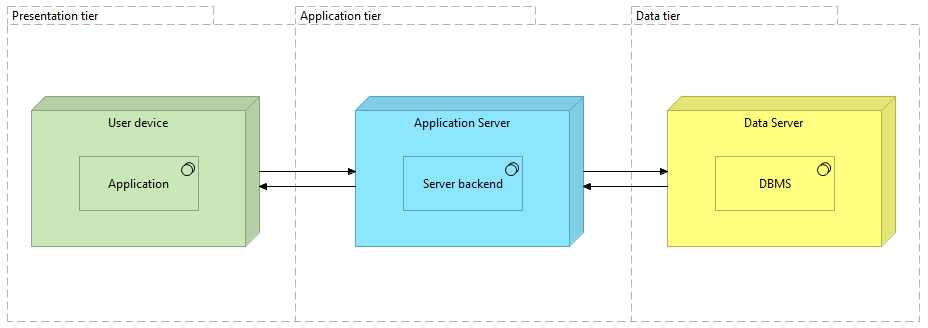
\includegraphics[width=\linewidth]{tier.png}
\end{figure}

SafeStreets system is organized as a three-tier layer, a standard design architecture used to provide a good level of security and performance thanks to subdivision of the tasks between the three tiers. Each tier runs on a different machine (or a group of machines with same structure), so that every tier is responsible of a specific task and the computational work is splitted between different machines, optimizing performances. This also improve the security of the system, because user devices needs to pass through the application server to access the data and have no way to directly access to it. 

Presentation tier runs directly on customers devices, that can be both smartphones running the official app or PCs using the web app, and its main goal is to handle the data and assets received by the application server to display the information on the device screen. User can then see the information requested and also interact with the presentation layer by using classical view widgets (like button, textfield, sliders ecc...) to require additional data based on their inputs. To summarize, main goals of presentation layer are communicating with the application server API to require data based on user input and visual the results on user's screen.

Application tier is composed by a replicated array of application servers, to scale horizontally the system using machines with the same structure and functionalities. The array of servers is managed by a load balancer, that distributes the clients' requests (and so the computational cost) equally between all the machines. Because application servers need to receive multiple requests from different clients in an effective way, load balancer integrate a router module that actively listens for any request made on specific server ports. The router has an handler for any endpoint of SafeStreets API that calls the manager related to the endpoint functionality, passing any input received in the request so that the manager can correctly consult or manipulate the database and produce an output, that is then returned by the router to the client that made that request. List of manager that fulfil the functionalities is reported in later section, in which every manager is also defined in detail.

Data tier task is to provide access to data to application tier, so that the manager modules can interrogate the database and also store or modify data in a reliable way. Data tier, like application tier, is composed by an array of replicated machine, with cloned databases that share memory disks. This structure helps in maintaining high performances while keeping the data safe from possible hardware issues or data loss.